
\documentclass[11pt]{article}


\usepackage{a4wide}
\usepackage{graphicx}


\begin{document}

\title{Pentesting Report: Smart WiFi Camera}
\author{Haohan Fu (), Jiayang Xu (2829543), Zhengyang Cheng (),
\\ Xi Wang (), Xibin Yu () and Haoyu Ju ()}
\date{12, March, 2025}
\maketitle







\section{Executive summary}

Give the high lights of your report, what are your key results and recommendations?

\section{High-level description of the device}

What is the device and what does it do? How does it work? Does it take commands, from a phone app? A cloud server? How does the user set it up? Etc.

The Goowls smart home camera, shown in figure 1:
\begin{figure}[htbp]
    \centering
    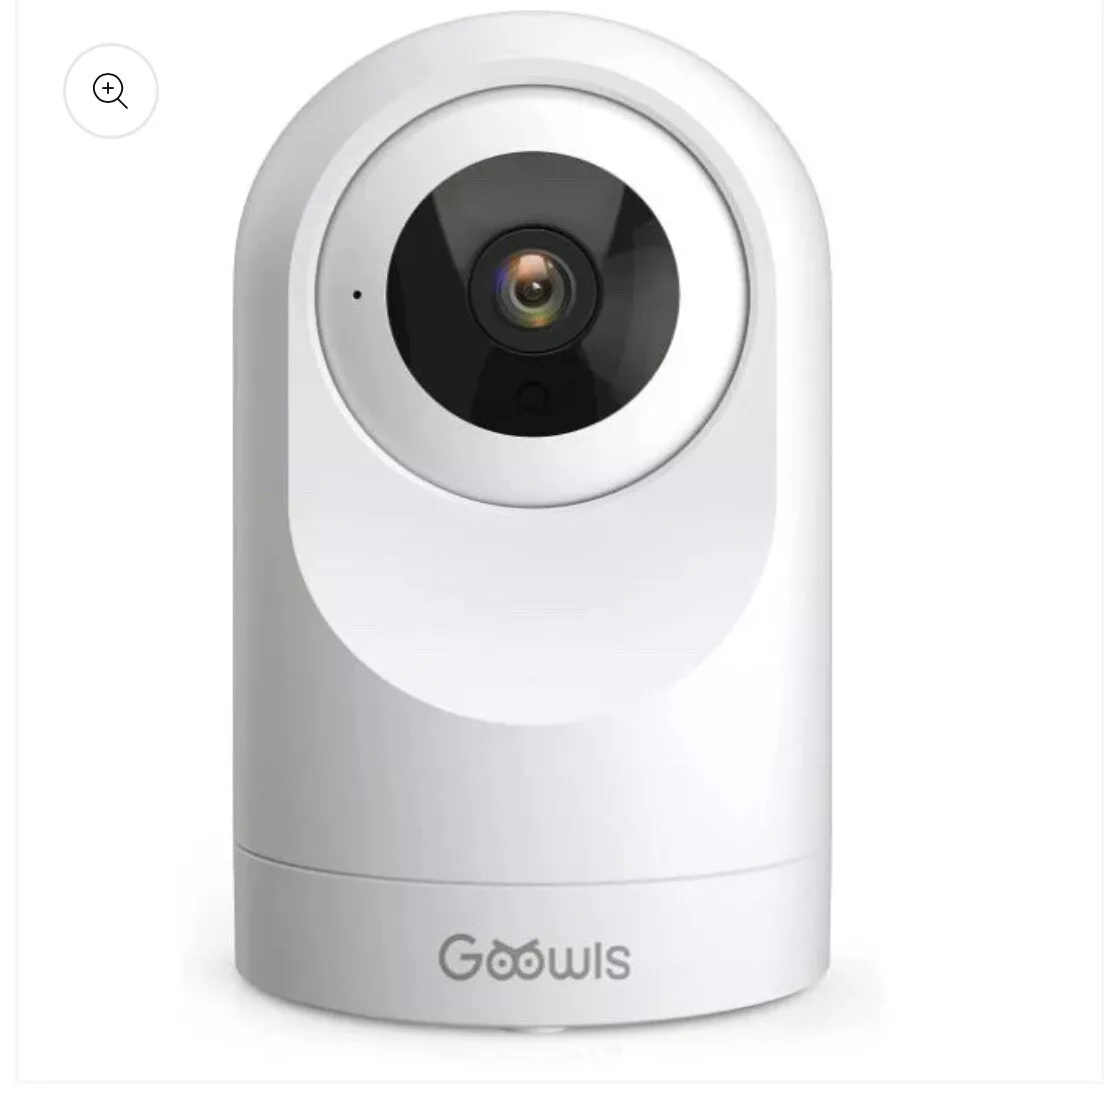
\includegraphics[width=0.5\textwidth]{imgs/camera.png}
    \caption{conponent of smart home camera}
\end{figure}

The Goowls Smart Home Camera is a versatile security device designed to enhance home monitoring. Users can integrate multiple Goowls cameras into their smart home ecosystem, allowing comprehensive surveillance across various areas of their residence.

Central to this system is the camera itself, which offers 1080p high-definition video quality for clear and detailed footage. Equipped with two-way audio, it enables real-time communication between the user and individuals near the camera. The device supports both local storage via a 4-64 GB Class 10 TF card and cloud storage options, providing flexibility in video recording management.

To operate the Goowls camera, users need to download the YI IoT app, available on both the Apple App Store and Google Play Store. Once installed and configured, the app allows users to view live video feeds, replay recorded footage, and receive motion detection alerts. Additionally, users can assign specific names to each camera's location (e.g., "Living Room" or "Nursery") for organized monitoring.

The Goowls camera is compatible with Amazon Alexa, enabling voice-controlled access to live feeds. To set up this feature, users must add the YI IoT skill to their Alexa app and link their account. Once connected, voice commands can be used to display camera feeds on Alexa-enabled devices.

\section{Investigating the device}

\subsection{Analysing the device setup}

Describe the technical details of how the device is set up by the user. What protocols are used and how? How did you fine this out? Give technical details, and enough information to ensure that your analysis is repeatable by someone else.

\subsection{Analysing the device in use}

Describe the technical details of how the device is used after set up. What protocols are used and how? How did you fine this out. Give technical details, and enough information to ensure that your analysis is repeatable by someone else.

\subsection{Analysing the apk file}

If you analysed the apk file, describe the app code and what you found.

\section{Possible attacks against the device}


\subsection{Attacks by a local attacker with wi-fi access}

What attacks are possible by an attacker with access to the same wi-fi network as the device? What could and couldnÕt such an attacker do and why? Describe both the possible attacks, if any, and also describe if the device provides defense from such an attacker, and say how. 

\subsection{Attacks by a local attacker without wi-fi access}

What attacks are possible by an attacker that is within wi-fi range of the device but does not have the wi-fi password? What could and couldnÕt such an attacker do and why? Describe both the possible attacks, if any, and also describe if the device provides defense from such an attacker, and say how. 

\subsection{Attacks by a remote attacker}

What attacks are possible by a remote attackers that can intercept and send messages on the Internet? What could and couldnÕt such an attacker do and why? Describe both the possible attacks, if any, and also describe if the device provides defense from such an attacker, and say how. 

\section{Analysis of the weaknesses found}

For each of the weaknesses you have found, describe the risk they pose to the owner of the device. What is the impact of the attacks? What would your advice be to someone that owned used such a device?


 
\appendix

\section{Additional technical information}

Include additional technical information to support your report. APK files, pcap files, Burp logs, a proof of concept attack code can be given to me on a USB stick.
\end{document}

